\subsection{实验目的}
学习和实践图像翻转、对数变换、幂次变换等图像处理方法。学习使用算术、逻辑操作实现图像增强。
\subsection{实验原理}
\subsubsection{图像反转}
对于二维灰度图像可以执行计算
\[ s=L-1-r \]
重新计算每一个像素点的像素值。这样计算之后得到的图像即为反转后的图像。图像反转会使得原本在图像中是明亮的区域变成黑暗的区域、黑暗的区域变成明亮的区域。
\subsubsection{对数变换}
对于二维灰度图像可以执行计算
\[ s=c\log(1+r) \]
重新计算每一点的像素值。这样的计算,可以提高图像在暗部或明部细节的辨识度。%例如,一个图像的能量主要集中在比较暗的部分,即在图像中暗部保存了许多细节,正常显示的时候会显得图像细节难以辨认。如果对这样的图像进行对数变换,那么就使得暗部的像素点的值得到提升,提高了图像在暗部的可辨识性。
\subsubsection{幂次变换}
对于二维的灰度图像可以执行计算
\[ s=cr^b \]
重新计算每一点的像素值。$c$和$b$为正常数,当$b$取不同值时将得到不同的变换曲线。
\subsubsection{使用算术、逻辑操作进行增强}
对两幅或多幅图像进行计算,进行求比值、求差值计算。可以实现从不同时期的遥感数据中分析出地表特征的变化。
\subsection{实验流程}
本次实验的实验流程如图\ref{fig:rsexp_flowchart}所示
\begin{figure}[H]
	\centering
\begin{tikzpicture}[node distance=1.4cm]
\node(start) [startstop] {开始};
\node(input_img) [io, below of=start] {读取二维灰度图片};
\node(power) [process, below of=input_img] {进行幂次变换};
\node(log) [process, below of=power] {进行对数变换};
\node(plot) [process, below of=log] {绘制变换曲线};
\node(output_img) [io, below of=plot] {输出变换后的图片};
\node(output_graph) [io, below of=output_img] {输出绘制的变换曲线};
\node(input_rsimg) [io, below of=output_graph] {读取具有差异的两幅遥感图像};
\node(process_rsimg) [process, below of=input_rsimg] {选择合适的变换对遥感图像进行处理};
\node(output_rsimg) [io, below of=process_rsimg] {输出处理后的遥感图像};
\node(end) [startstop, below of=output_rsimg] {结束};

\draw[arrow] (start) -- (input_img);
\draw[arrow] (input_img) -- (power);
\draw[arrow] (power) -- (log);
\draw[arrow] (log) -- (plot);
\draw[arrow] (plot) -- (output_img);
\draw[arrow] (output_img) -- (output_graph);
\draw[arrow] (output_graph) -- (input_rsimg);
\draw[arrow] (input_rsimg) -- (process_rsimg);
\draw[arrow] (process_rsimg) -- (output_rsimg);
\draw[arrow] (output_rsimg) -- (end);
\end{tikzpicture}
\caption{图像变换实验流程图}
\label{fig:rsexp_flowchart}
\end{figure}
\subsection{实验程序}
\lstinputlisting[caption={反转变换程序代码}]{"../Executable Script/Exp 2/ReverseTransformAndCompare.m"}
\lstinputlisting[caption={反转变换函数}]{"../Function Library/ReverseTransform.m"}
\lstinputlisting[caption={反转变函数曲线绘制代码}]{"../Executable Script/Exp 2/PlotReverseTransformFunction.m"}
\lstinputlisting[caption={幂次变换程序代码}]{"../Executable Script/Exp 2/GammaTransformAndCompare.m"}
\lstinputlisting[caption={幂次变换函数}]{"../Function Library/GammaTransform.m"}
\lstinputlisting[caption={幂次变换函数曲线绘制函数}]{"../Function Library/PlotGammaTransformFunction.m"}
\lstinputlisting[caption={对数变换程序代码}]{"../Executable Script/Exp 2/LogTransformAndCompare.m"}
\lstinputlisting[caption={对数变换函数}]{"../Function Library/LogTransform.m"}
\lstinputlisting[caption={对数变换函数曲线绘制函数}]{"../Function Library/PlotLogTransformFunction.m"}
\lstinputlisting[caption={遥感图像变化检测}]{"../Executable Script/Exp 2/CompareTwoImages.m"}
\lstinputlisting[caption={自动二值化图像函数}]{"../Function Library/AutoBinarizeImage.m"}
\subsection{实验结果和分析}
\begin{figure}[H]
	\centering
	\begin{minipage}{0.45\linewidth}
		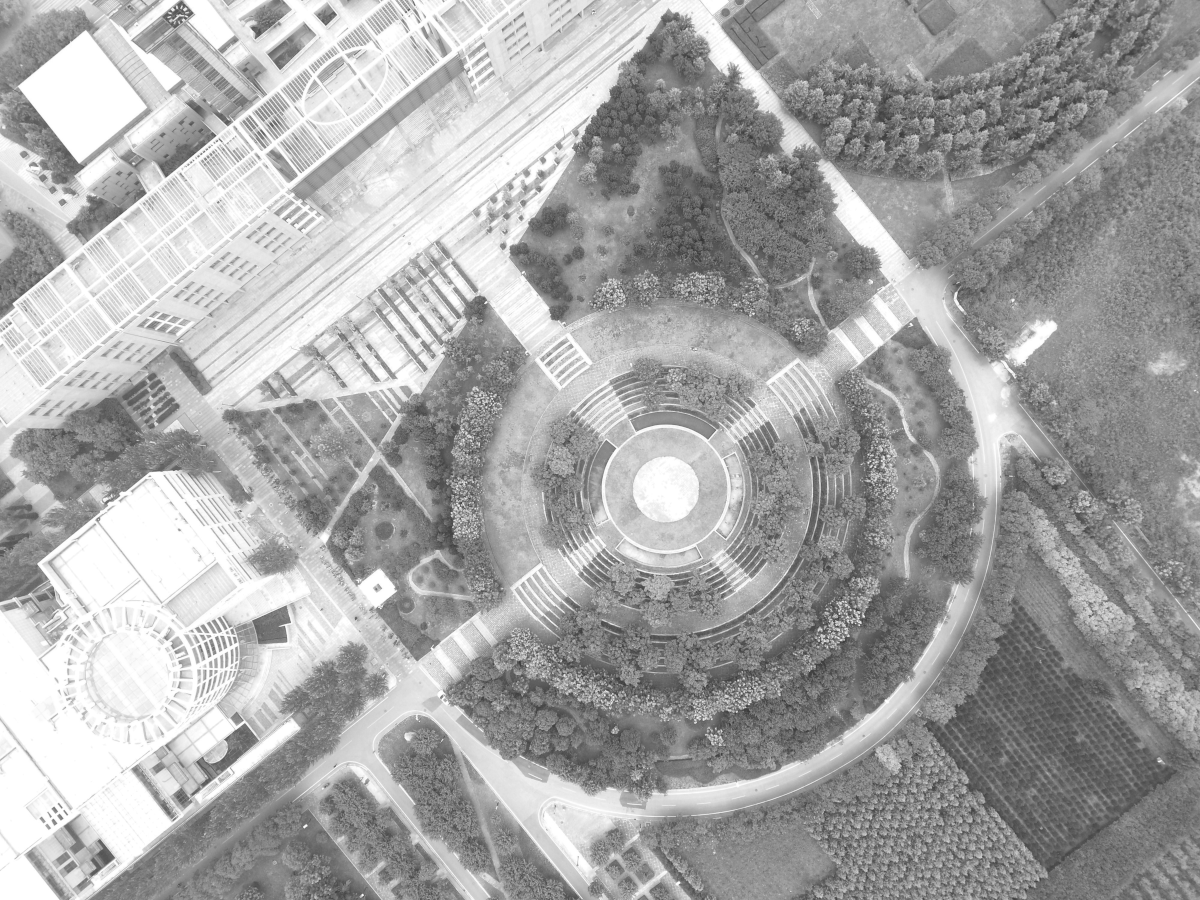
\includegraphics[width=\linewidth]{figure/DJI_0027_Gray.png}
		\caption{原图片}
		\label{fig:transform_original}
	\end{minipage}
	\begin{minipage}{0.45\linewidth}
		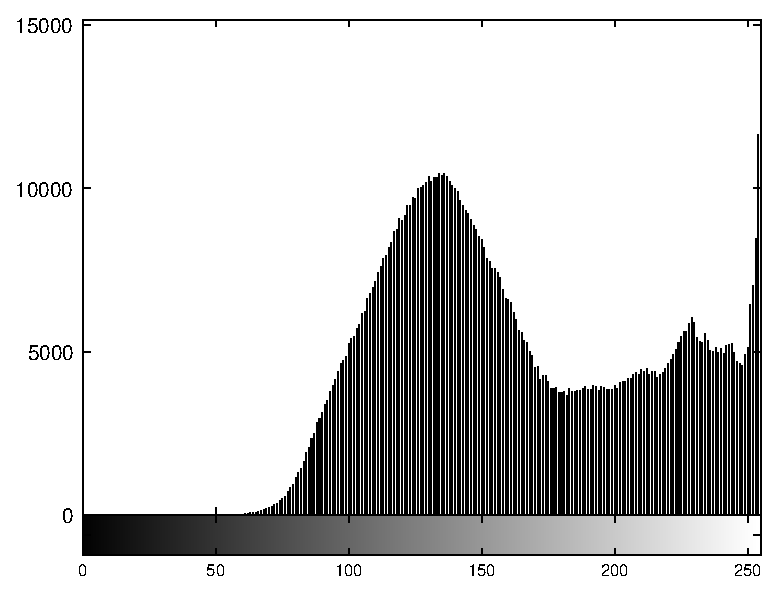
\includegraphics[width=\linewidth]{figure/DJI_0027_Histogram}
		\caption{原图片统计直方图}
		\label{fig:dji0027histogram}
	\end{minipage}
\end{figure}
\subsubsection{反转变换}
\begin{figure}[H]
	\centering
	\begin{minipage}{0.45\linewidth}
		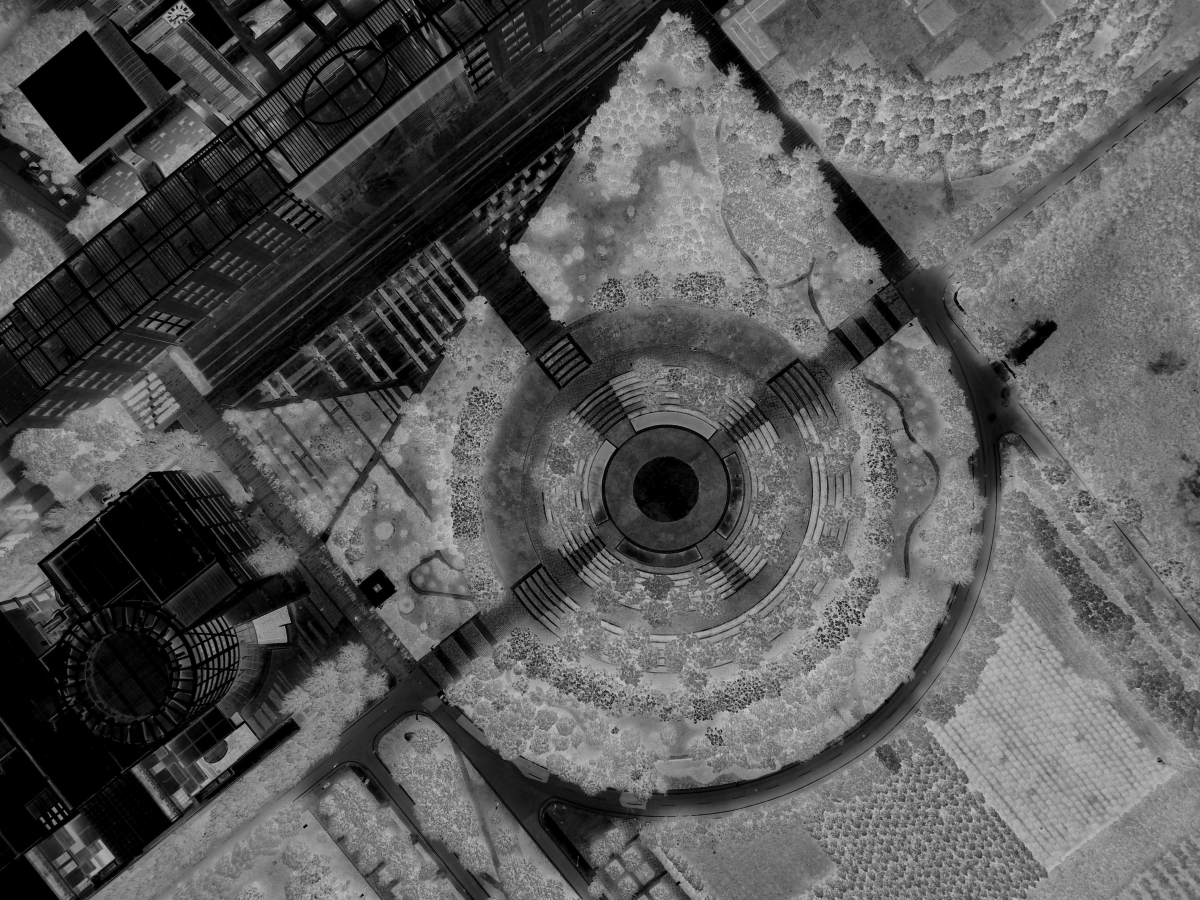
\includegraphics[width=\linewidth]{figure/DJI_0027_Reversed.png}
		\caption{$s=L-1-r$的反转变换}
	\end{minipage}
	\begin{minipage}{0.45\linewidth}
		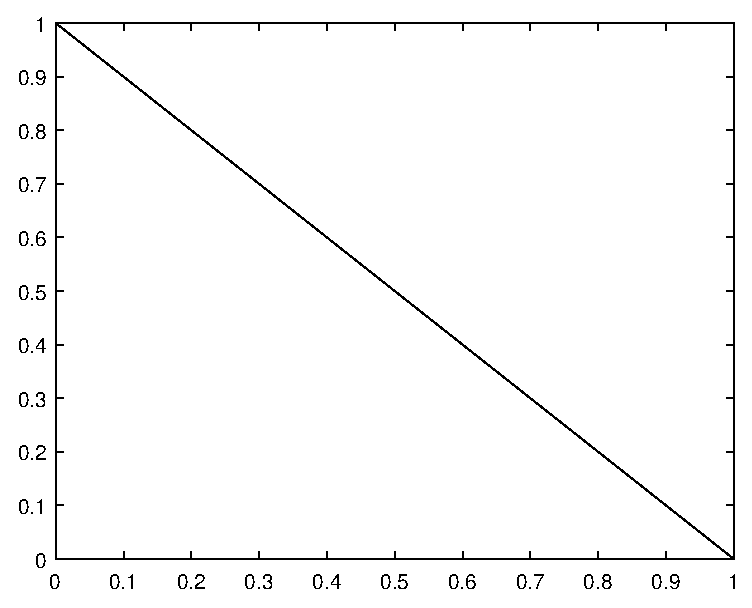
\includegraphics[width=\linewidth]{figure/DJI_0027_Reversed_Graph.eps}
		\caption{$s=L-1-r$变换曲线}
	\end{minipage}
\end{figure}
\subsubsection{幂次变换}
$b=1$的幂次变换
\begin{figure}[H]
	\centering
	\begin{minipage}{0.45\linewidth}
		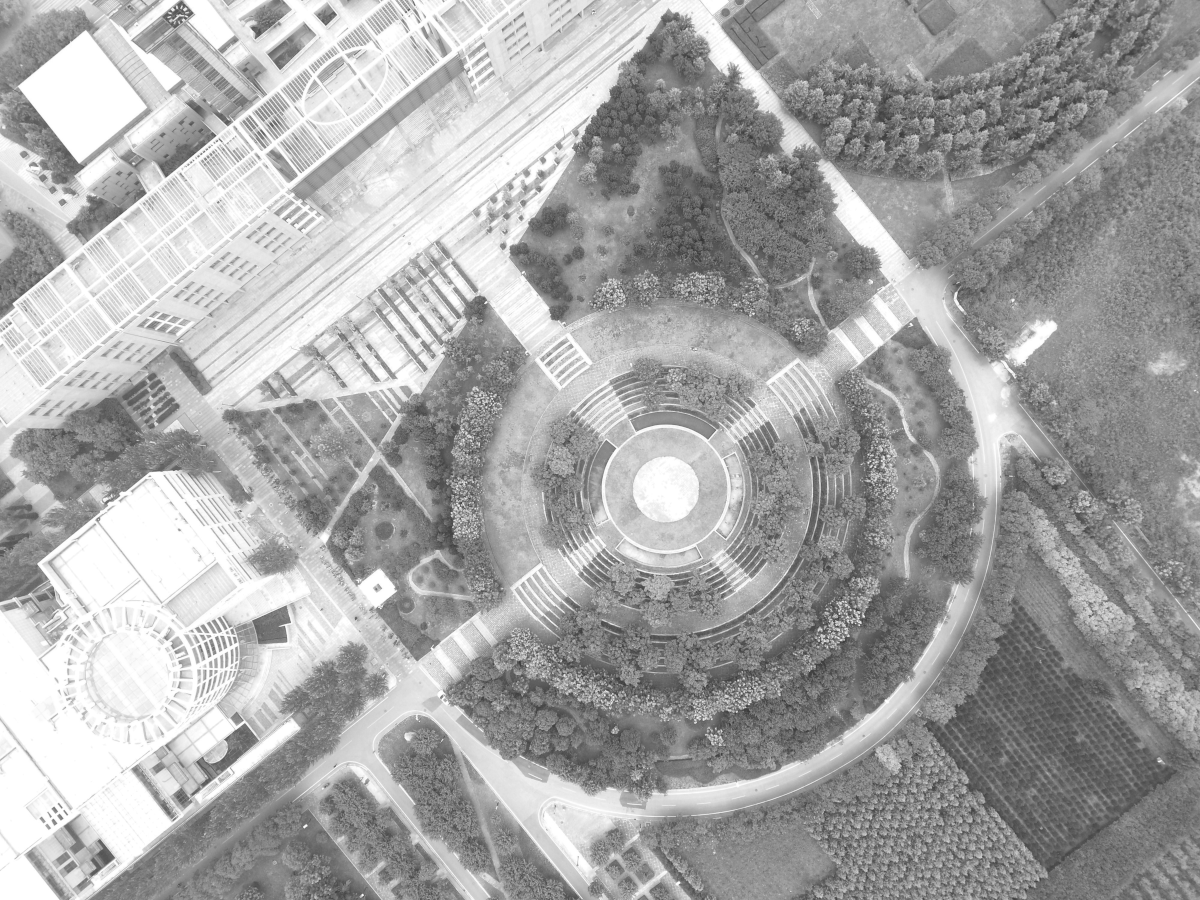
\includegraphics[width=\linewidth]{figure/DJI_0027_Gamma_100.png}
		\caption{$s=1r^1$的幂次变换}
	\end{minipage}
	\begin{minipage}{0.45\linewidth}
		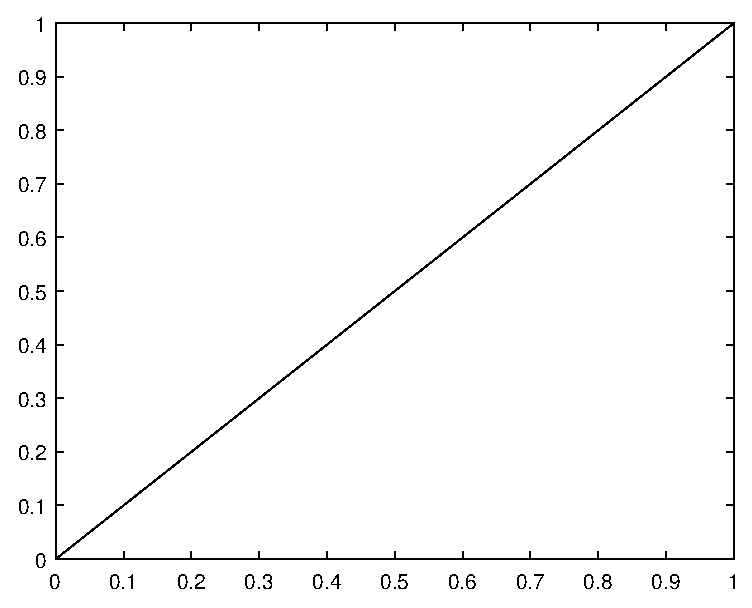
\includegraphics[width=\linewidth]{figure/DJI_0027_Gamma_100_Graph.eps}
		\caption{$s=1r^1$变换曲线}
	\end{minipage}
\end{figure}

$b=0.5$的幂次变换
\begin{figure}[H]
	\centering
	\begin{minipage}{0.45\linewidth}
		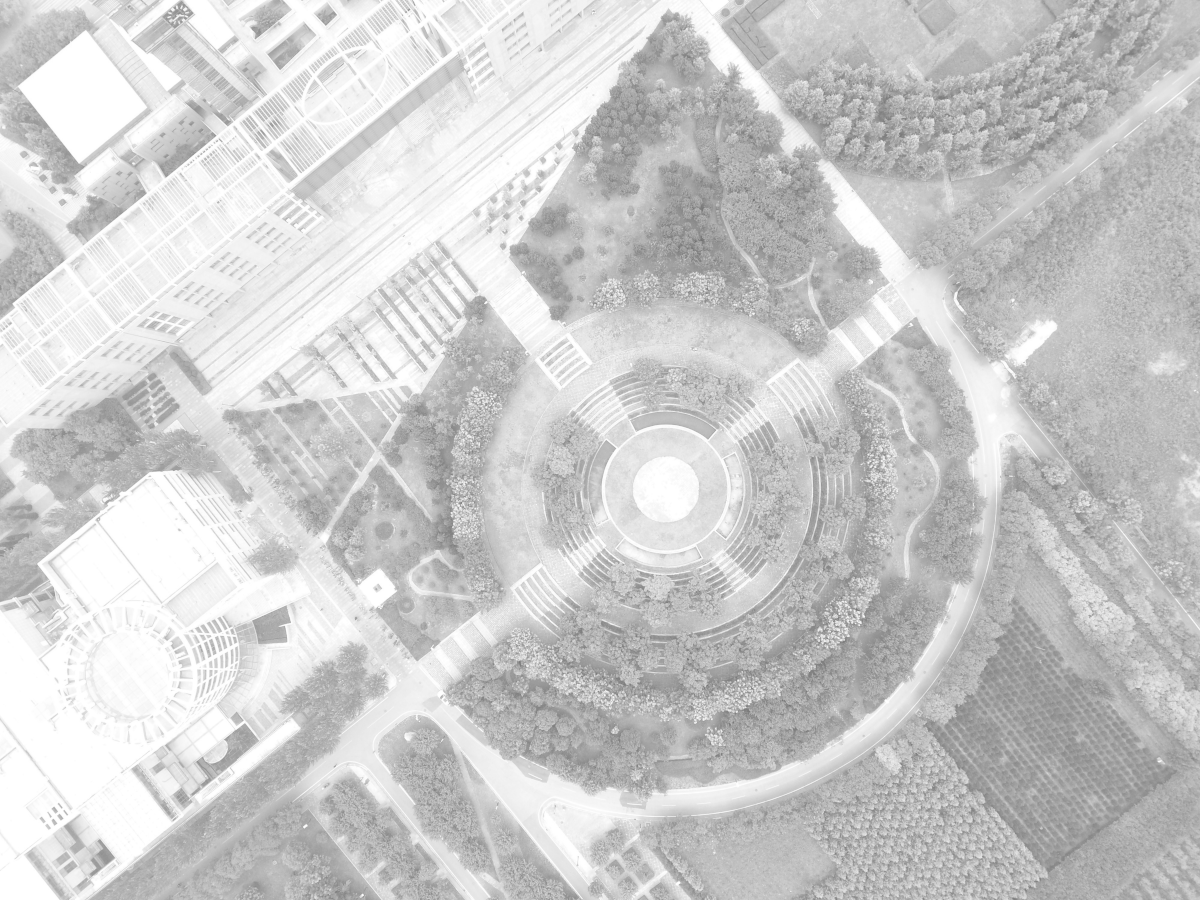
\includegraphics[width=\linewidth]{figure/DJI_0027_Gamma_50.png}
		\caption{$s=1r^{0.5}$的幂次变换}
	\end{minipage}
	\begin{minipage}{0.45\linewidth}
		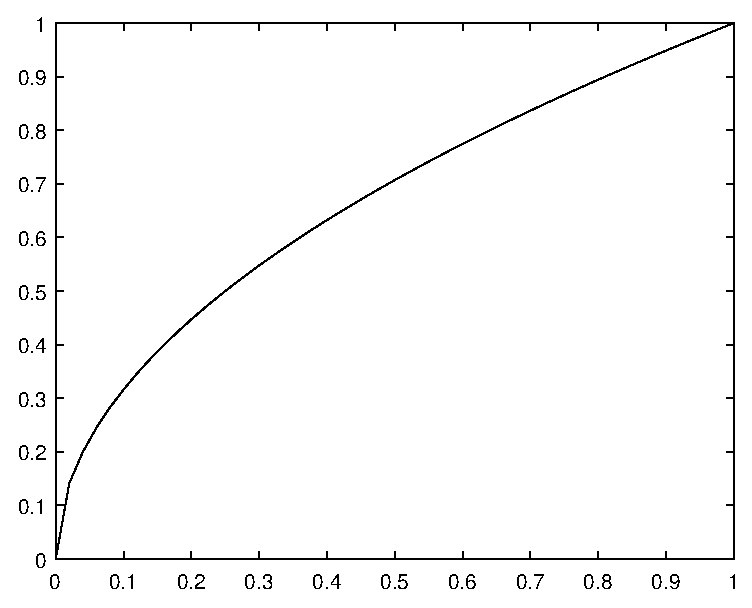
\includegraphics[width=\linewidth]{figure/DJI_0027_Gamma_50_Graph.eps}
		\caption{$s=1r^{0.5}$变换曲线}
	\end{minipage}
\end{figure}

$b=2$的幂次变换
\begin{figure}[H]
	\centering
	\begin{minipage}{0.45\linewidth}
		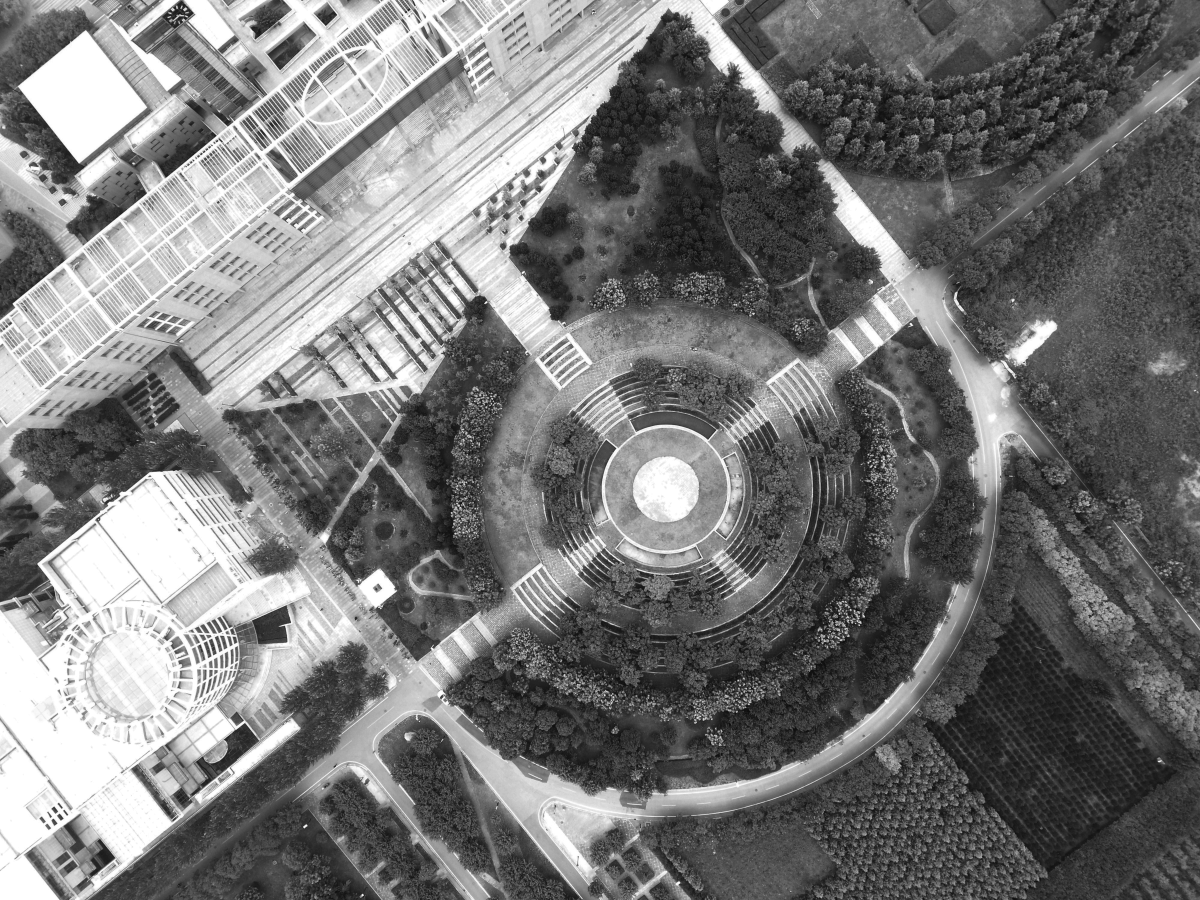
\includegraphics[width=\linewidth]{figure/DJI_0027_Gamma_200.png}
		\caption{$s=1r^2$的幂次变换}
	\end{minipage}
	\begin{minipage}{0.45\linewidth}
		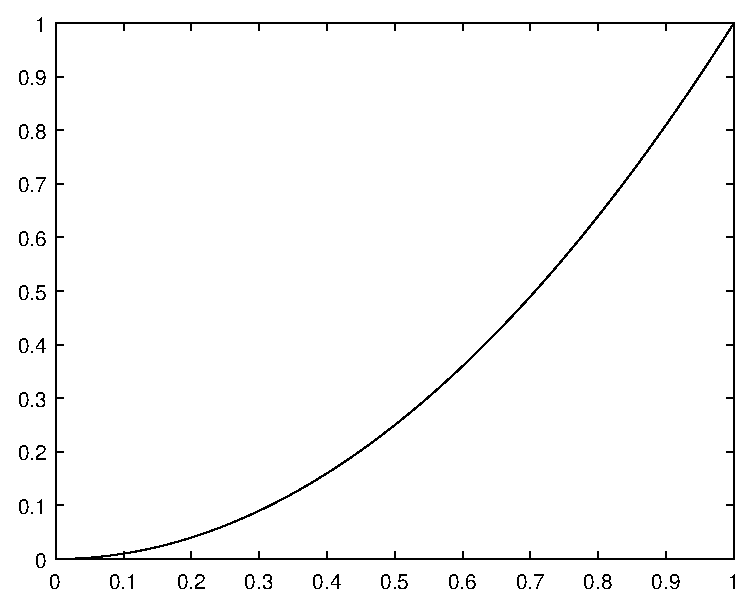
\includegraphics[width=\linewidth]{figure/DJI_0027_Gamma_200_Graph.eps}
		\caption{$s=1r^2$变换曲线}
	\end{minipage}
\end{figure}
\subsubsection{对数变换}
$c=1$的对数变换
\begin{figure}[H]
	\centering
	\begin{minipage}{0.45\linewidth}
		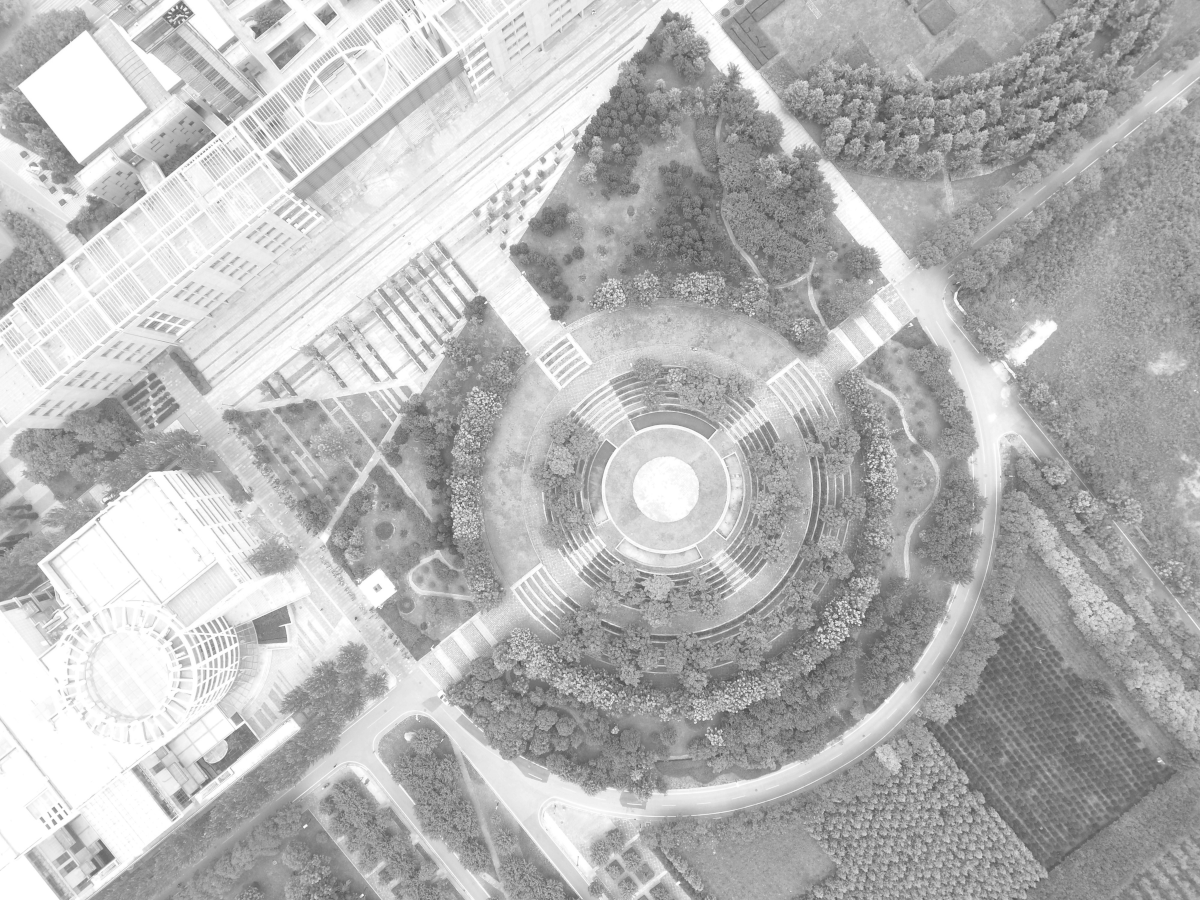
\includegraphics[width=\linewidth]{figure/DJI_0027_Log_100.png}
		\caption{$s=\log_2(1+1r)$的对数变换}
	\end{minipage}
	\begin{minipage}{0.45\linewidth}
		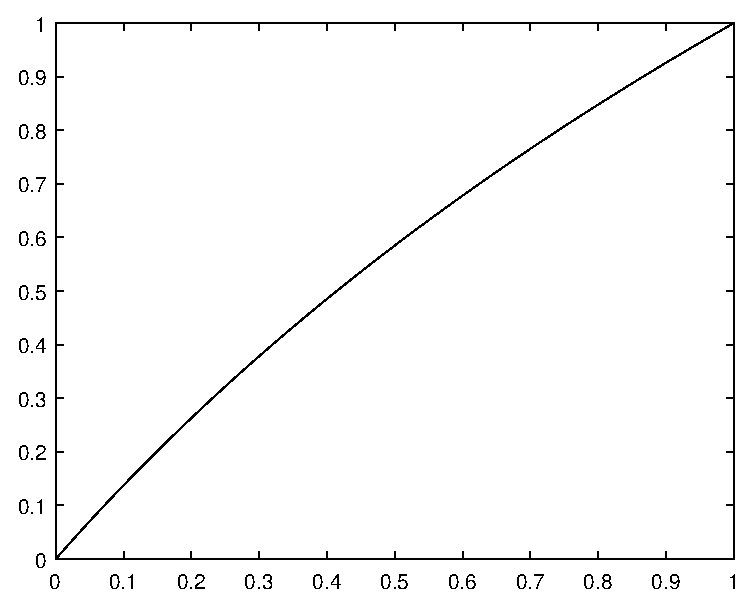
\includegraphics[width=\linewidth]{figure/DJI_0027_Log_100_Graph.eps}
		\caption{$s=\log_2(1+1r)$变换曲线}
	\end{minipage}
\end{figure}

$c=10$的对数变换
\begin{figure}[H]
	\centering
	\begin{minipage}{0.45\linewidth}
		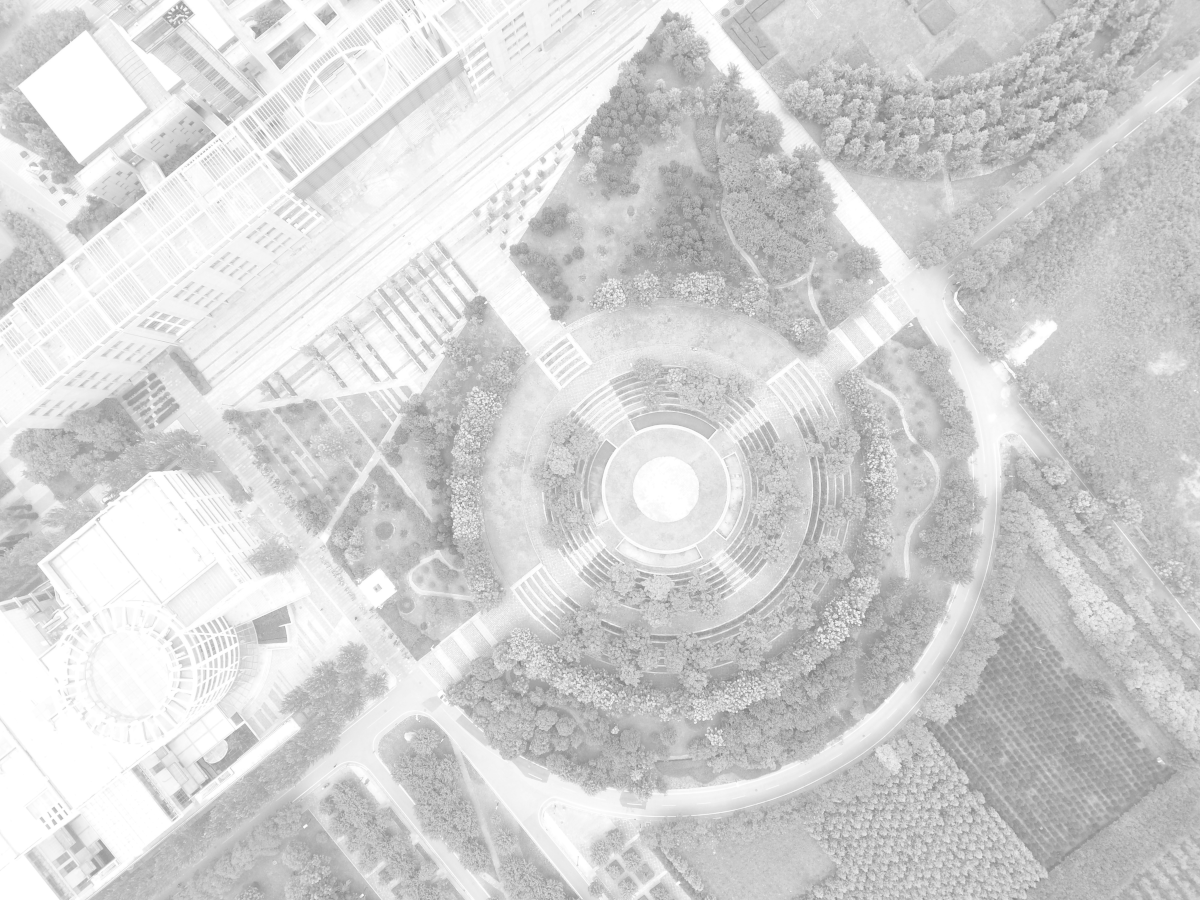
\includegraphics[width=\linewidth]{figure/DJI_0027_Log_1000.png}
		\caption{$s=\log_{11}(1+10r)$的对数变换}
	\end{minipage}
	\begin{minipage}{0.45\linewidth}
		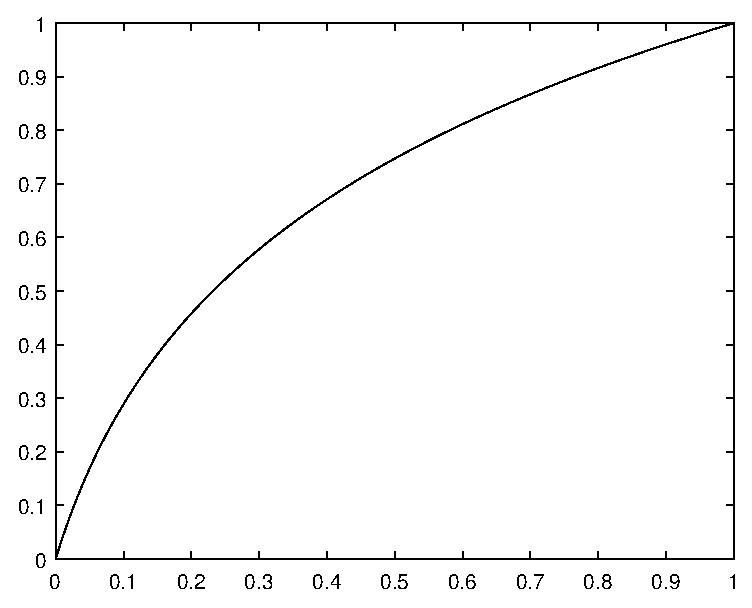
\includegraphics[width=\linewidth]{figure/DJI_0027_Log_1000_Graph.eps}
		\caption{$s=\log_{11}(1+10r)$变换曲线}
	\end{minipage}
\end{figure}

$c=-0.9$的对数变换
\begin{figure}[H]
	\centering
	\begin{minipage}{0.45\linewidth}
		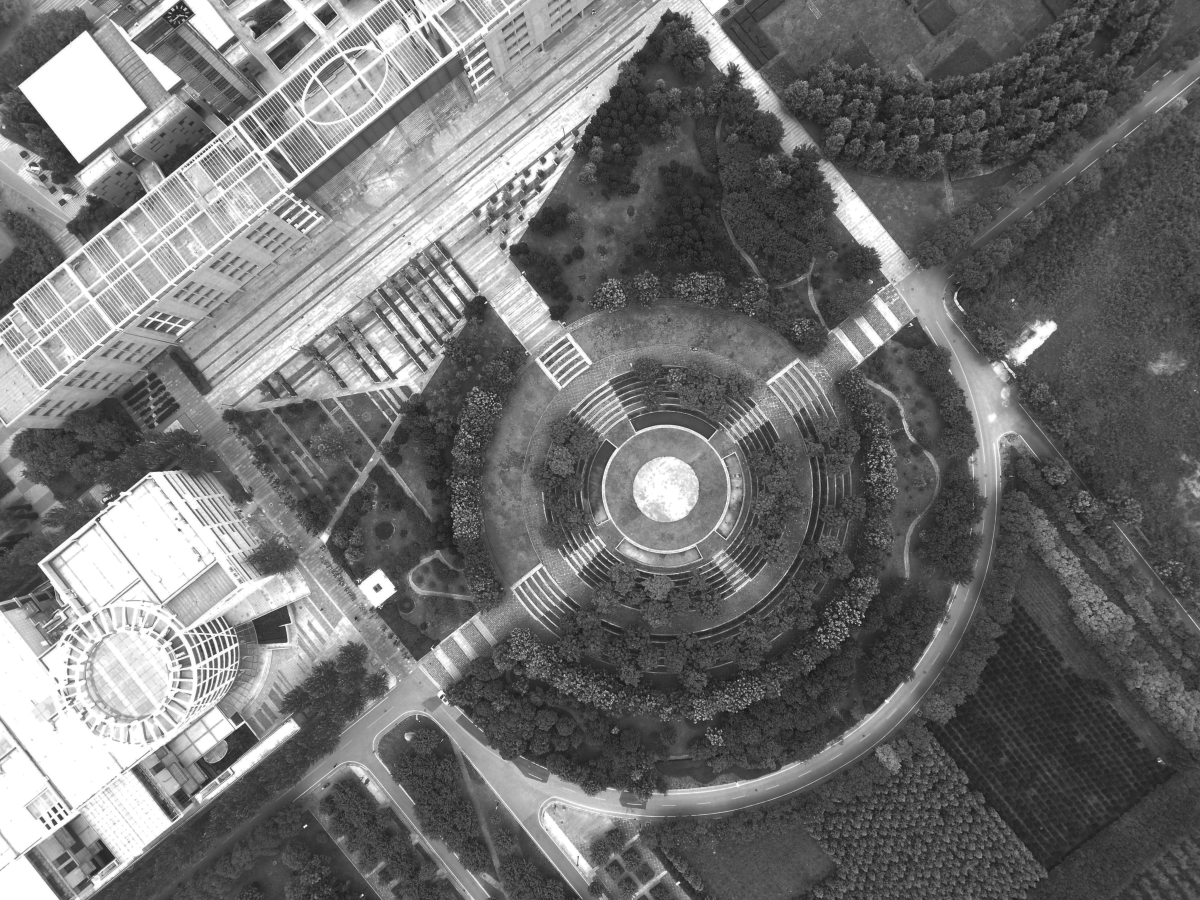
\includegraphics[width=\linewidth]{figure/DJI_0027_Log_-90.png}
		\caption{$s=\log_{0.1}(1-0.9r)$的对数变换}
	\end{minipage}
	\begin{minipage}{0.45\linewidth}
		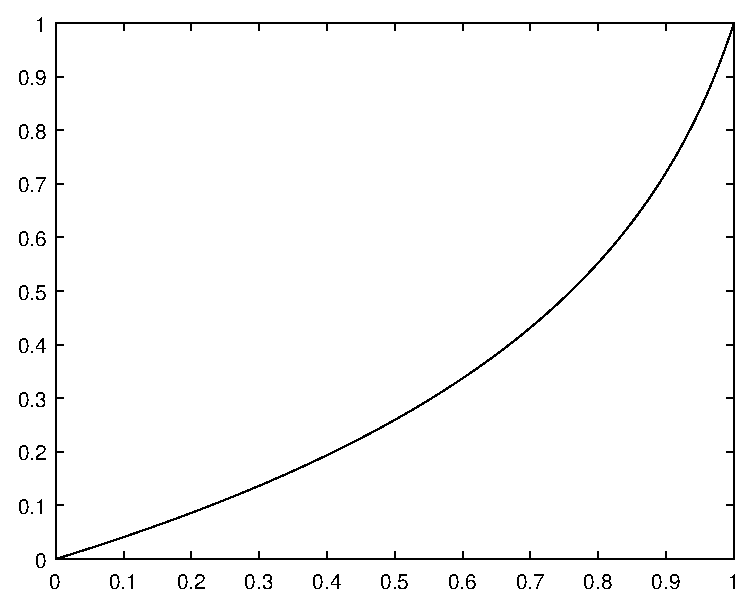
\includegraphics[width=\linewidth]{figure/DJI_0027_Log_-90_Graph.eps}
		\caption{$s=\log_{0.1}(1-0.9r)$变换曲线}
	\end{minipage}
\end{figure}
\subsubsection{遥感图像变化检测}
\begin{figure}[H]
	\centering
	\begin{minipage}{0.45\linewidth}
		\includegraphics[width=\linewidth]{figure/san_gt.bmp}
		\caption{示例变化检测}
	\end{minipage}
	\begin{minipage}{0.45\linewidth}
		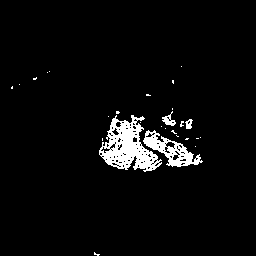
\includegraphics[width=\linewidth]{figure/exp2compare.png}
		\caption{自主实现的变化检测}
	\end{minipage}
\end{figure}
对不同参数、不同变换类型进行比较可以发现,当变换曲线为凹函数时,即对于变换函数$f(x)$,在$\left[0, 1 \right] $内,均有$f''(x)>0$,则在变换后的图像中,暗部取值被压缩,亮部取值范围展宽,能更好突出图像亮部细节;当变换曲线为凸函数时,即对于变换函数$f(x)$,在$\left[0, 1 \right] $内,均有$f''(x)<0$,则在变换后的图像中,亮部取值被压缩,暗部取值范围展宽,能更好地突出图像暗部细节。所以对图像进行处理时应进行灵活的选择,要根据目标及其周围的明暗特征选择合适的变换曲线,以更好地突出目标的特征。

在幂次变换中$s=cr^b$,其中$b$的取值会影响变换曲线的凹凸性和变化率。从图像变换的结果中可以看出,当$0<b<1$时,变换曲线为凸函数,$b$的取值越小,变换曲线在暗部越陡峭、明部越平缓;当$b=1$时,变换曲线为正比例函数,图像不发生变化;当$b>1$时,变换曲线为凹函数,$b$的取值越大,变换曲线在明部越陡峭、暗部越平缓;当$b\leq 0$时,将会出现计算错误导致不正常的输出。